% !TeX root = Report.tex
\documentclass[12pt]{article}

% Package imports (organized and deduplicated)
\usepackage{biblatex}
\usepackage{changepage}
\usepackage{color}
\usepackage{enumitem}
\usepackage{float}
\usepackage{graphicx}
\usepackage{listings}
\usepackage{sectsty}
\usepackage{xcolor}
\usepackage[breaklinks=true]{hyperref}
\usepackage{xurl}
\usepackage{tikz}
\usepackage{lipsum}
\usepackage[format=plain,
            labelfont=it,
            textfont=]{caption}
\usetikzlibrary{shapes.geometric, arrows, positioning, calc}
\usepackage{./timing-diagrams}
\usetikzlibrary{calc}
\setcounter{biburlnumpenalty}{100}
\setcounter{biburlucpenalty}{100}
\setcounter{biburllcpenalty}{100}

\newcommand{\subsubsubsection}[1]{\paragraph{#1}\mbox{}\\}
\setcounter{secnumdepth}{4}
\setcounter{tocdepth}{4}

\newcommand{\writersnote}[1]{\marginpar{\small{\textcolor{blue}{Writer's note:}} \scriptsize\textit{#1}}}

% \usepackage{background}
% \backgroundsetup{
%   position=current page.north west,
%   angle=0,
%   nodeanchor=north west,
%   vshift=-1cm,
%   hshift=1cm,
%   color=red,
%   opacity=1,
%   scale=1,
%   contents={Preprint}
% }

\definecolor{darkblue}{RGB}{0, 0, 102} 
\hypersetup{
    colorlinks=true,
    pdfborder={0 0 0},
    linkbordercolor=white,
    urlcolor=darkblue,
    linkcolor=darkblue,
    citecolor=darkblue,
    filecolor=darkblue
}

% Make bibliography ragged right instead of justified
\AtBeginDocument{
  \renewcommand{\bibsetup}{\raggedright}
}
% Document configuration
\restylefloat{table}
\graphicspath{{./images/}}
\addbibresource{Library.bib}
\subsectionfont{\fontsize{12}{14}\selectfont}

% Author information
\author{
    Group Number: 107\\
    Joar Heimonen, Christian Vu, Naly Keli \\
    \texttt{contact@joar.me}\\ 
    \texttt{chvu002@student.kristiania.no}\\
    \texttt{nake002@student.kristiania.no}
}

% Title configuration
\title{
  \textbf{Preliminary Title}\\
  \large{Preliminary Description}
}
\date{\today}

\newcommand{\license}{
    \vspace{1em}
    \noindent\small{© 2025 Joar Heimonen,  Christian Vu, Naly Keli\\
    This work is licensed under a \href{https://creativecommons.org/licenses/by-sa/4.0/}{Creative Commons Attribution-Sharealike 4.0 International License}.}
}
\begin{document}
\maketitle

\begin{abstract}
  Preliminary Abstract
\end{abstract}

\pagebreak

\tableofcontents

\pagebreak


\section{Introduction}
There are many paradigms of commercial sensor management and monitoring. Organizations can use anything from 
PLC (programmable Logic Controllers) to IoT devices to manage and monitor their sensors. For commercial use 
some of these alternatives are more popular than others. There are also a large amount of different higher level protocols
like MQTT, HTTP and SNMP that can be used to manage and monitor sensors. We propose using the NETCONF protocol 
with YANG sensor models for management. This work will be done in collaboration with Lightside Instruments AS.

\writersnote{
  unprecise, replace: "can use anything from..." and all other vague statements.
}

This document will cover the following three topics:
\begin{itemize}
  \item \textbf{Work methodology:} An indept analysis of the knowledge base around work methods like Scrum, Kanban, and Waterfall. 
  With a focus on how our work methodology differs from these.
  \item \textbf{NETCONF and YANG sensor management}: A qualitative analysis of the NETCONF and YANG protocols and how they can be used to manage sensors.
  \item \textbf{NETCONF Security}: A qualitative analysis of the security aspects of the NETCONF protocol.
\end{itemize}

\section{Lightside Instruments AS}
Lightside Instruments is a company specializing in developing instruments with model based network management 
for use in networking, network interconnect testing and telemetry. 
They design their instruments with YANG (RFC7950) models and NETCONF (RFC6241) \cite{ennsNetworkConfigurationProtocol2011} protocol. 
The instruments are based on IETF standards and drafts, 
and are implemented with software tools available in Debian, programmable 
logic and open hardware. \cite{LightsideInstrumentsYANG}

\section{Technical background}

\subsection{NETCONF and YANG}
NETCONF \cite{ennsNetworkConfigurationProtocol2011} is a model based Network Configuration Protocol.
Each NETCONF device presents the aquiring device with a YANG \cite{bjorklundYANG11Data2016} data model
consisting of the device state and parameters. 
Each data model has a set of constraints making them error correcting.

\section{Work methodology}

\subsection{Research Question}
This meta study examines the claims that Scrum, Kanban, Waterfall, Extreme Programming and DevOps 
increases worker productivity substantiated by empirical evidence.


\subsection{Scoping Review}
\subsubsection{Search strategy}
The following is our search strategy for the scoping review.
We will be searching for quantitative studies on the efficiency of the following work methodologies:
\begin{itemize}
  \item Scrum
  \item Kanban
  \item Waterfall
  \item Extreme Programming
  \item DevOps
\end{itemize}
We will be searching the following databases:
\begin{itemize}
  \item IEEE Xplore \cite{IEEEXplore}
  \item ACM Digital Library \cite{ACMDigitalLibrary}
  \item Google Scholar \cite{GoogleScholar} (Meta database)
\end{itemize}
We will also be searching the following industry websites:
\begin{itemize}
  \item Agile Alliance \cite{AgileAlliance2015}
  \item Scrum.org \cite{HomeScrumorg}
  \item DevOps Institute \cite{Organisations}
  \item Scrum Alliance \cite{ScrumAllianceFind}
\end{itemize}
Our search will consists of a set of primary and secondary keywords.
The primary keywords are:
\begin{itemize}
  \item Scrum
  \item Kanban
  \item Waterfall
  \item Extreme Programming
  \item DevOps
\end{itemize}
The secondary keywords are:
\begin{itemize}
  \item Effectiveness
  \item Efficiency
  \item Productivity
  \item Performance
  \item Success
  \item Failure
\end{itemize}
The search will be done using the following search string:

\begin{adjustwidth}{-4em}{0pt}
\begin{verbatim}
       (Scrum OR Kanban OR Waterfall OR "Extreme Programming" OR DevOps) 
                                      AND
(Effectiveness OR Efficiency OR Productivity OR Performance OR Success OR Failure)
\end{verbatim}
\end{adjustwidth}

\subsubsection{Inclusion and Exclusion Criteria}
The systematic review will include peer-reviewed articles meeting the following criteria:
\begin{itemize}
  \item Published after January 1, 2020
  \item Evaluating the effectiveness of the following methodologies:
  \begin{itemize}
    \item Scrum
    \item Kanban
    \item Waterfall
    \item Extreme Programming
    \item DevOps
  \end{itemize}
\end{itemize}


\subsubsection{PRISMA flow diagram}

\begin{figure}
  \centering
 \begin{adjustwidth}{-4em}{0pt}
 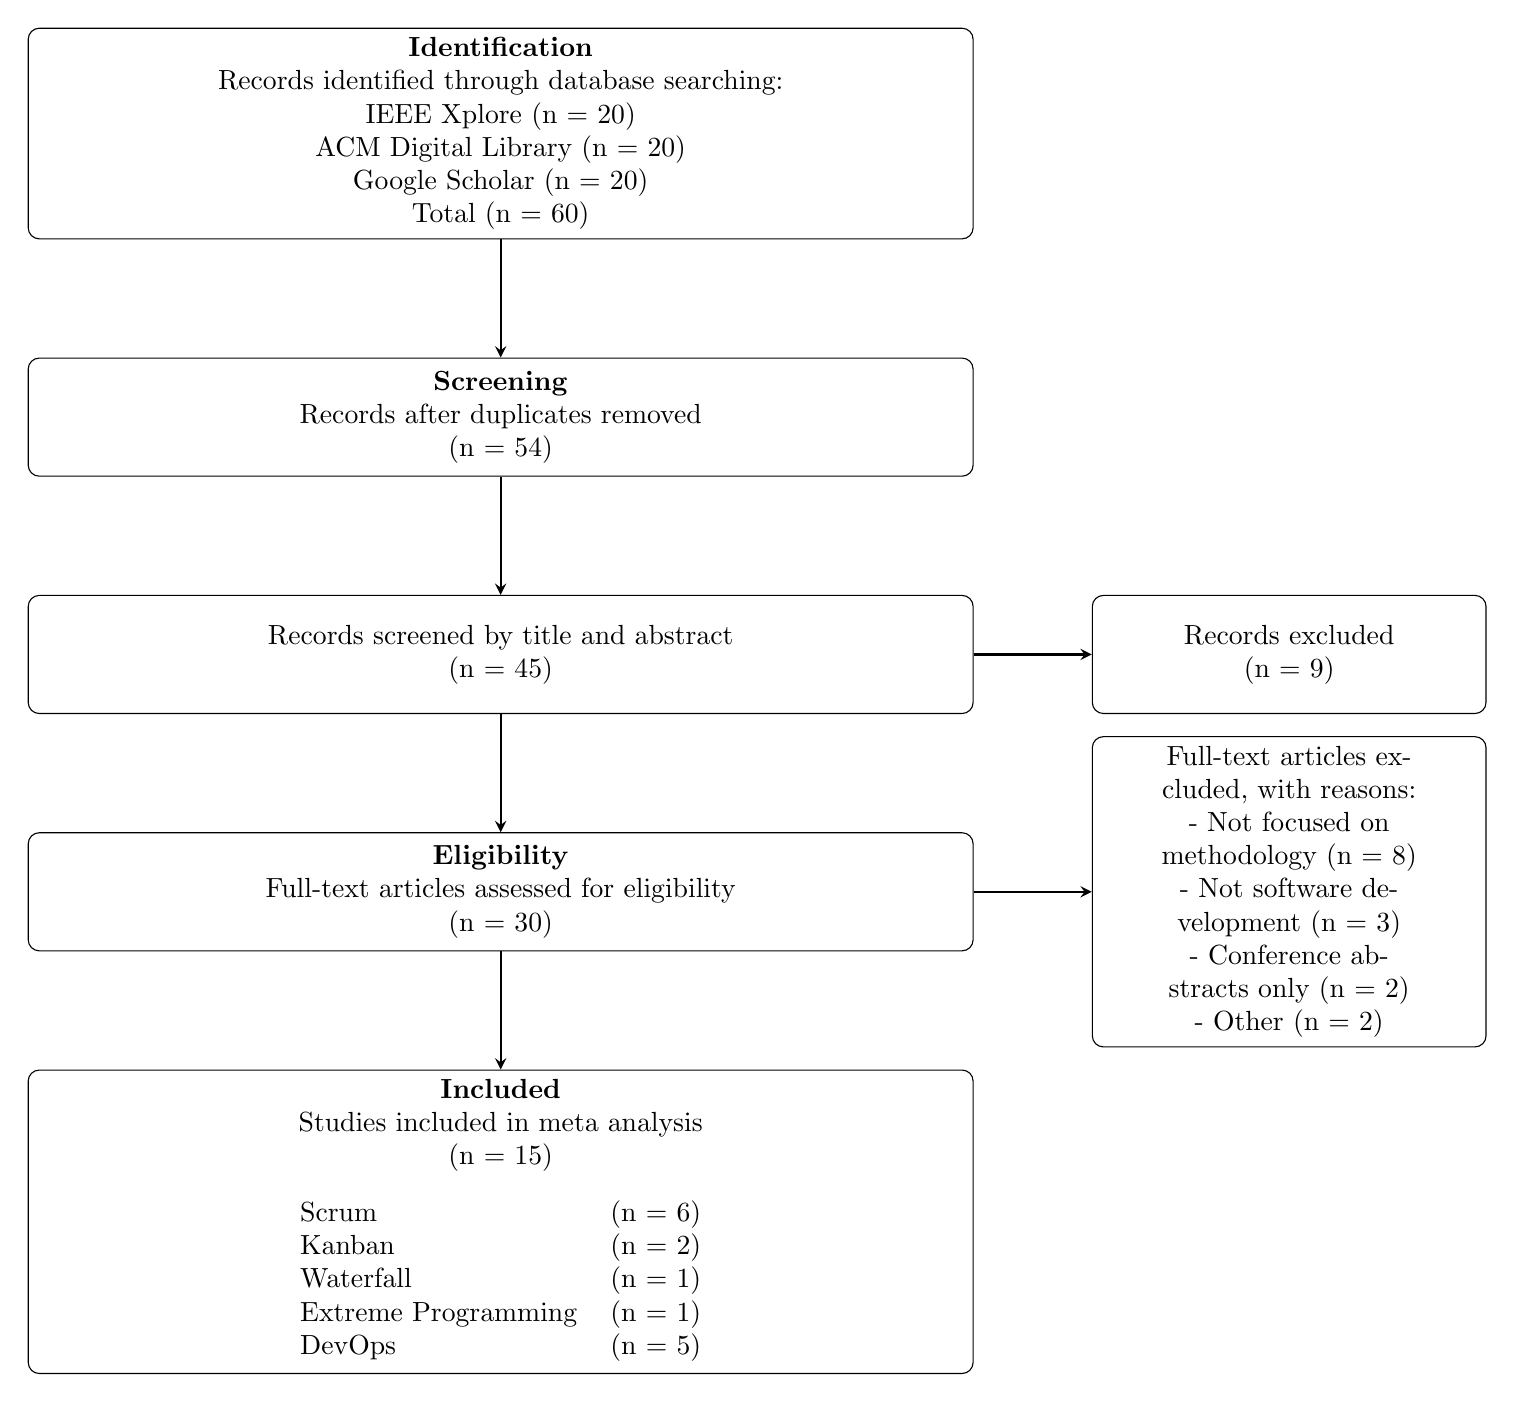
\begin{tikzpicture}[
  node distance = 1.5cm,
  box/.style = {draw, rectangle, rounded corners, minimum width=12cm, minimum height=1.5cm, text width=11.5cm, align=center},
  sidebox/.style = {draw, rectangle, rounded corners, minimum width=5cm, minimum height=1.5cm, text width=4.5cm, align=center},
  line/.style = {draw, -stealth, thick}
  ]
 % Identification box
 \node[box] (identification)
  {\textbf{Identification} \\
  Records identified through database searching:\\
  IEEE Xplore (n = 20)\\
  ACM Digital Library (n = 20)\\
  Google Scholar (n = 20)\\
  Total (n = 60)};
 % Screening boxes
 \node[box, below=of identification] (screening1)
  {\textbf{Screening} \\
  Records after duplicates removed\\
  (n = 54)};
 \node[box, below=of screening1] (screening2)
  {Records screened by title and abstract\\
  (n = 45)};
 \node[sidebox, right=1.5cm of screening2] (excluded1)
  {Records excluded\\
  (n = 9)};
 % Eligibility boxes
 \node[box, below=of screening2] (eligibility)
  {\textbf{Eligibility} \\
  Full-text articles assessed for eligibility\\
  (n = 30)};
 \node[sidebox, right=1.5cm of eligibility] (excluded2)
  {Full-text articles excluded, with reasons:\\
  - Not focused on methodology (n = 8)\\
  - Not software development (n = 3)\\
  - Conference abstracts only (n = 2)\\
  - Other (n = 2)};
 % Included box
 \node[box, below=of eligibility] (included)
  {\textbf{Included} \\
  Studies included in meta analysis\\
  (n = 15)\\[0.3cm]
 \begin{tabular}{ll}
  Scrum & (n = 6)\\
  Kanban & (n = 2)\\
  Waterfall & (n = 1)\\
  Extreme Programming & (n = 1)\\
  DevOps & (n = 5)
 \end{tabular}};
 % Arrows
 \draw[line] (identification) -- (screening1);
 \draw[line] (screening1) -- (screening2);
 \draw[line] (screening2) -- (eligibility);
 \draw[line] (eligibility) -- (included);
 \draw[line] (screening2) -- (excluded1);
 \draw[line] (eligibility) -- (excluded2);
 \end{tikzpicture}
 \end{adjustwidth}
 \caption{PRISMA \cite{PRISMAStatement} flow diagram for scoping review of software development methodologies}
 \label{fig:prisma}
 \end{figure}


\subsection{Scrum}


\subsection{Kanban}
\subsection{Waterfall}
\subsection{Extreme Programming}
\subsection{DevOps}


\section{NETCONF and YANG sensor management}

\subsection{Node RED}
\subsubsection{node-yuma123}
\subsubsubsection{easyNetconf}

\section{NETCONF Security}

\pagebreak
\addcontentsline{toc}{section}{References}
\printbibliography
\license
\end{document}
